\documentclass{article}

\usepackage{fancyhdr}
\usepackage{extramarks}
\usepackage{amsmath}
\usepackage{amsthm}
\usepackage{amsfonts}
\usepackage{tikz}
\usepackage{graphicx} %插入图片的宏包
\usepackage{float} %设置图片浮动位置的宏包
\usepackage{pythonhighlight}
% \usepackage{subfigure} %插入多图时用子图显示的宏包
% \usepackage[plain]{algorithm}
% \usepackage{algpseudocode}

% \usetikzlibrary{automata,positioning}

%
% Basic Document Settings
%

\topmargin=-0.45in
\evensidemargin=0in
\oddsidemargin=0in
\textwidth=6.5in
\textheight=9.0in
\headsep=0.25in

\linespread{1.1}

\pagestyle{fancy}
\lhead{\hmwkAuthorName}
\chead{\hmwkClass\ : \hmwkTitle}
\rhead{\firstxmark}
\lfoot{\lastxmark}
\cfoot{\thepage}

\renewcommand\headrulewidth{0.4pt}
\renewcommand\footrulewidth{0.4pt}

\setlength\parindent{0pt}


%代码格式设置



%
% Create Problem Sections
%

\newcommand{\enterProblemHeader}[1]{
    \nobreak\extramarks{}{Problem \arabic{#1} continued on next page\ldots}\nobreak{}
    \nobreak\extramarks{Problem \arabic{#1} (continued)}{Problem \arabic{#1} continued on next page\ldots}\nobreak{}
}

\newcommand{\exitProblemHeader}[1]{
    \nobreak\extramarks{Problem \arabic{#1} (continued)}{Problem \arabic{#1} continued on next page\ldots}\nobreak{}
    \stepcounter{#1}
    \nobreak\extramarks{Problem \arabic{#1}}{}\nobreak{}
}

\setcounter{secnumdepth}{0}
\newcounter{partCounter}
\newcounter{homeworkProblemCounter}
\setcounter{homeworkProblemCounter}{1}
\nobreak\extramarks{Problem \arabic{homeworkProblemCounter}}{}\nobreak{}

%
% Homework Problem Environment
%
% This environment takes an optional argument. When given, it will adjust the
% problem counter. This is useful for when the problems given for your
% assignment aren't sequential. See the last 3 problems of this template for an
% example.
%
\newenvironment{homeworkProblem}[1][-1]{
    \ifnum#1>0
        \setcounter{homeworkProblemCounter}{#1}
    \fi
    \section{Problem \arabic{homeworkProblemCounter}}
    \setcounter{partCounter}{1}
    \enterProblemHeader{homeworkProblemCounter}
}{
    \exitProblemHeader{homeworkProblemCounter}
}

%
% Homework Details
%   - Title
%   - Due date
%   - Class
%   - Section/Time
%   - Instructor
%   - Author
%

\newcommand{\hmwkTitle}{Quiz\ \#12}
\newcommand{\hmwkDueDate}{Jan 27th, 2019}
\newcommand{\hmwkClass}{Complex Networks}
\newcommand{\hmwkClassTime}{Section A}
% \newcommand{\hmwkClassInstructor}{Professor Isaac Newton}
\newcommand{\hmwkAuthorName}{\textbf{RUOPENG XU} }
\newcommand{\hmwkAuthorNum}{\textbf{18M38179} }

%
% Title Page
%

\title{
    \vspace{2in}
    \textmd{\textbf{\hmwkClass:\ \hmwkTitle}}\\
    \normalsize\vspace{0.1in}\small{Due\ on\ \hmwkDueDate\ }\\
    % \vspace{0.1in}\large{\textit{\hmwkClassInstructor\ \hmwkClassTime}}
    \vspace{3in}
}

\author{\hmwkAuthorName\\ \hmwkAuthorNum}
\date{}

\renewcommand{\part}[1]{\textbf{\large Part \Alph{partCounter}}\stepcounter{partCounter}\\}

%
% Various Helper Commands
%

% Useful for algorithms
\newcommand{\alg}[1]{\textsc{\bfseries \footnotesize #1}}

% For derivatives
\newcommand{\deriv}[1]{\frac{\mathrm{d}}{\mathrm{d}x} (#1)}

% For partial derivatives
\newcommand{\pderiv}[2]{\frac{\partial}{\partial #1} (#2)}

% Integral dx
\newcommand{\dx}{\mathrm{d}x}

% Alias for the Solution section header
\newcommand{\solution}{\textbf{\large Solution}}

% Probability commands: Expectation, Variance, Covariance, Bias
\newcommand{\E}{\mathrm{E}}
\newcommand{\Var}{\mathrm{Var}}
\newcommand{\Cov}{\mathrm{Cov}}
\newcommand{\Bias}{\mathrm{Bias}}

\begin{document}

\maketitle

\pagebreak

\begin{homeworkProblem}
    % questions
1.Plot the degree distributions of (a) Erdos-Renyi graph and (b) Barabasi-Albert graph of 10,000 nodes and about 50,000 edges. 

% 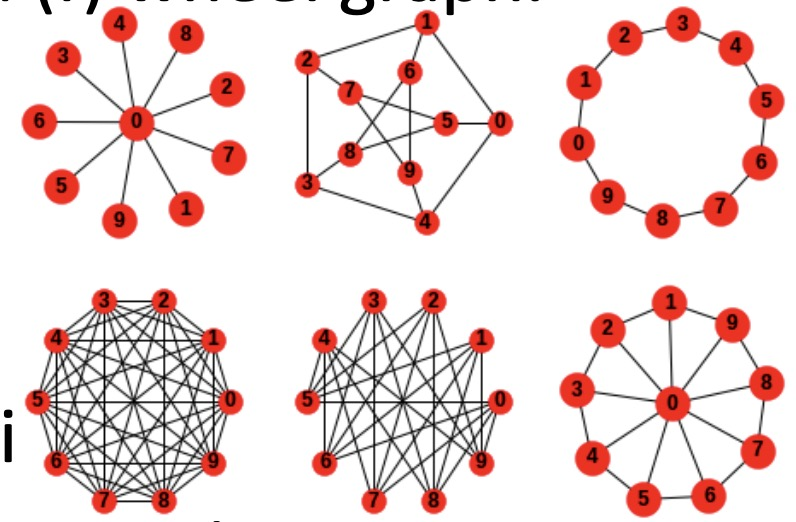
\includegraphics[scale=0.3]{quiz6_1.jpg}

\subsection*{Answer 1}


\begin{python}
import collections
import matplotlib.pyplot as plt
import networkx as nx

ba = nx.barabasi_albert_graph(10000, 5) #only this line is changed
print(nx.info(ba))

degree_sequence = sorted([d for n, d in ba.degree()], reverse=True)  # degree sequence
# print("Degree sequence", degree_sequence)
degreeCount = collections.Counter(degree_sequence)
deg, cnt = zip(*degreeCount.items())

fig, ax = plt.subplots()
plt.bar(deg, cnt, width=0.80, color='b')

plt.title("Degree Histogram of BA")
plt.ylabel("Count")
plt.xlabel("Degree")
ax.set_xticks([d + 0.4 for d in deg])
ax.set_xticklabels(deg)

plt.show()



er = nx.erdos_renyi_graph(10000, 0.001)#only this line is changed
print(nx.info(er))

degree_sequence = sorted([d for n, d in er.degree()], reverse=True)  # degree sequence
# print("Degree sequence", degree_sequence)
degreeCount = collections.Counter(degree_sequence)
deg, cnt = zip(*degreeCount.items())

fig, ax = plt.subplots()
plt.bar(deg, cnt, width=0.80, color='b')

plt.title("Degree Histogram of ER")
plt.ylabel("Count")
plt.xlabel("Degree")
ax.set_xticks([d + 0.4 for d in deg])
ax.set_xticklabels(deg)


plt.show()
\end{python}

The result is:\\
\begin{python}
Name: 
Type: Graph
Number of nodes: 10000
Number of edges: 49975
Average degree:   9.9950
\end{python}
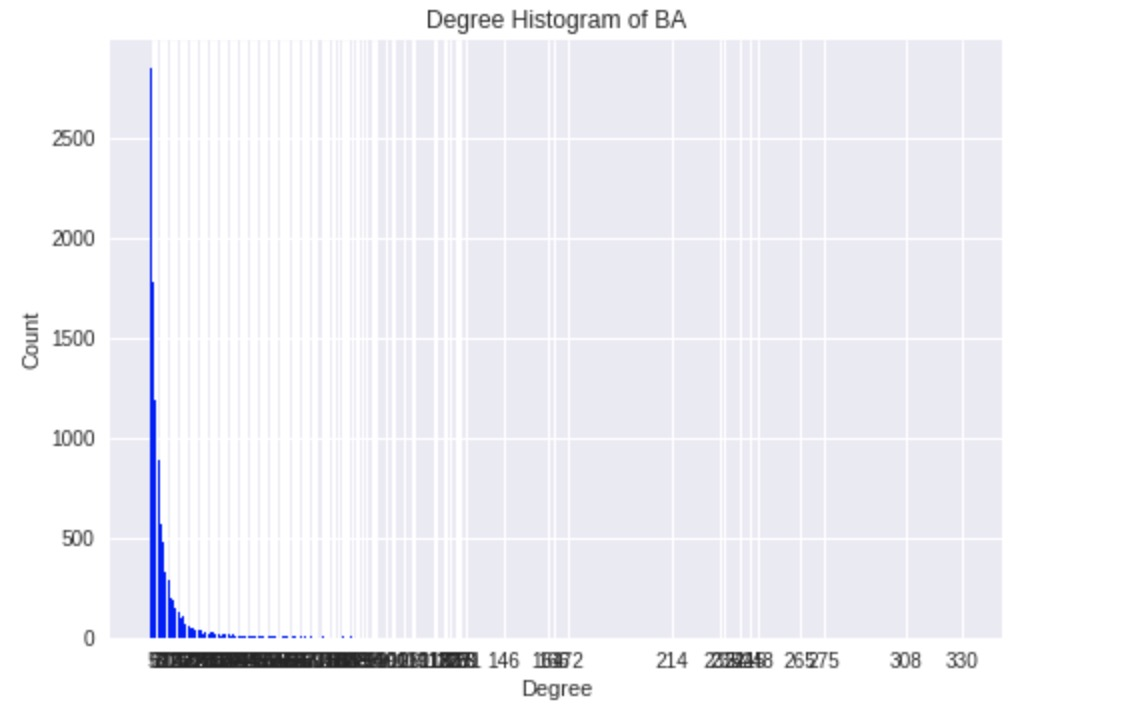
\includegraphics[scale=0.4]{quiz12_1.jpg}
\begin{python}
Name: 
Type: Graph
Number of nodes: 10000
Number of edges: 49931
Average degree:   9.9862
\end{python}
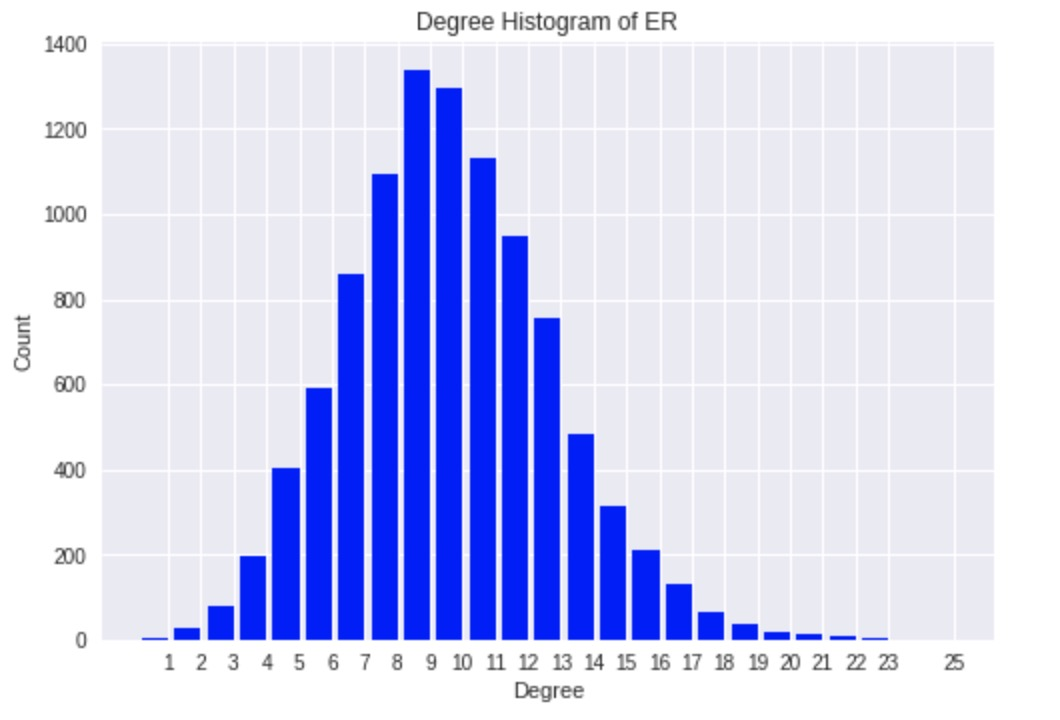
\includegraphics[scale=0.4]{quiz12_2.jpg}



\end{homeworkProblem}
\pagebreak

\begin{homeworkProblem}
2. Show the following metrics of the above both graphs.\\
• Number of nodes\\
• Number of edges\\
• Average degree\\
• Number of connected components\\
• Number of triangles\\
• Transitivity (clustering coefficient)\\
• Maximum degree\\
• Minimum degree\\

\subsection*{Answer 2}
\begin{python}
import networkx as nx
#import numpy as np
import matplotlib.pyplot as plt
from networkx.utils.random_sequence import powerlaw_sequence

er = nx.erdos_renyi_graph(10000, 0.001)
print("Erdos-Renyi graph")
print(nx.info(er))
print("connected components:", nx.number_connected_components(er))
sum1 = 0
for i in range(0,10000):
  sum1 = sum1 + nx.triangles(er, i)
print("numer of triangles:",int(sum1/3))
print("transitivity:",nx.transitivity(er))
er_degree_sequence = sorted([d for n, d in er.degree()], reverse=True)
print("max degree:",max(er_degree_sequence))
print("min degree:",min(er_degree_sequence))

print()
ba = nx.barabasi_albert_graph(10000, 5)
print("Barabasi-Albert graph")
print(nx.info(ba))
print("connected components:", nx.number_connected_components(ba))
sum2 = 0
for i in range(0,10000):
  sum2 = sum2 + nx.triangles(ba, i)
print("numer of triangles:",int(sum2/3))
print("transitivity:",nx.transitivity(ba))
ba_degree_sequence = sorted([d for n, d in ba.degree()], reverse=True)
print("max degree:",max(ba_degree_sequence))
print("min degree:",min(ba_degree_sequence))
\end{python}

The result is :
\begin{python}
Erdos-Renyi graph
Name: 
Type: Graph
Number of nodes: 10000
Number of edges: 50170
Average degree:  10.0340
connected components: 1
numer of triangles: 167
transitivity: 0.0009979761601223865
max degree: 23
min degree: 1

Barabasi-Albert graph
Name: 
Type: Graph
Number of nodes: 10000
Number of edges: 49975
Average degree:   9.9950
connected components: 1
numer of triangles: 2451
transitivity: 0.005371160091688837
max degree: 439
min degree: 5
\end{python}


\end{homeworkProblem}
\pagebreak


\end{document}
%
% Non sequential homework problems
%

% Jump to problem 18
